\chapter{Estado del arte}
Existen diferentes alternativas para controlar robots o microcontroladores
de forma remota, muchas de estas se agrupan bajo la denominación
``Internet of Things'', en este capítulo se describirán algunas de las
más destacadas y las más similares a XRemoteBot.

% FIXME: mmmm NO SE SI ESTO DEBERÍA ESTAR EN UN CAPITULO APARTE.....  LO HABLAMOS LUEGO

\section{Educabot}
El proyecto Educabot~\footnote{\url{http://www.educabot.org/}} tiene por
objetivos enseñar tecnología a niños y adultos a través
del uso, programación y construcción de robots. En el sitio del proyecto
se ofertan cursos orientados a los distintos niveles, estos robots se
usaron en actividades en distintas escuelas de la Ciudad Autónoma de Buenos
Aires~\footnote{\url{https://youtu.be/1oCOAtX9OS4}}.

% FIXME: ES ORIGINARIO DE ..... EN ESCUELAS? EN ONGS? DONDE SE LOS USA?
% Son cursos privados según dijo el tipo, pero no tengo de donde citar
% eso no dice nada el sitio.

En la parte de construcción este proyecto plantea un modelo de robot denominado
``Rolo'' para los jóvenes de más de 10 años, mientras que para los más chicos
se plantean actividades con el robot ``elBrian'' que incluyen
controlarlo a través de una interfaz Web que muestra las imágenes emitidas
por la cámara incorporada en este robot y además permite controlarlo con
botones en pantalla que determinan en qué dirección debe moverse el robot
(figura~\ref{fig:elbrian}).

\begin{figure}
    \centering
    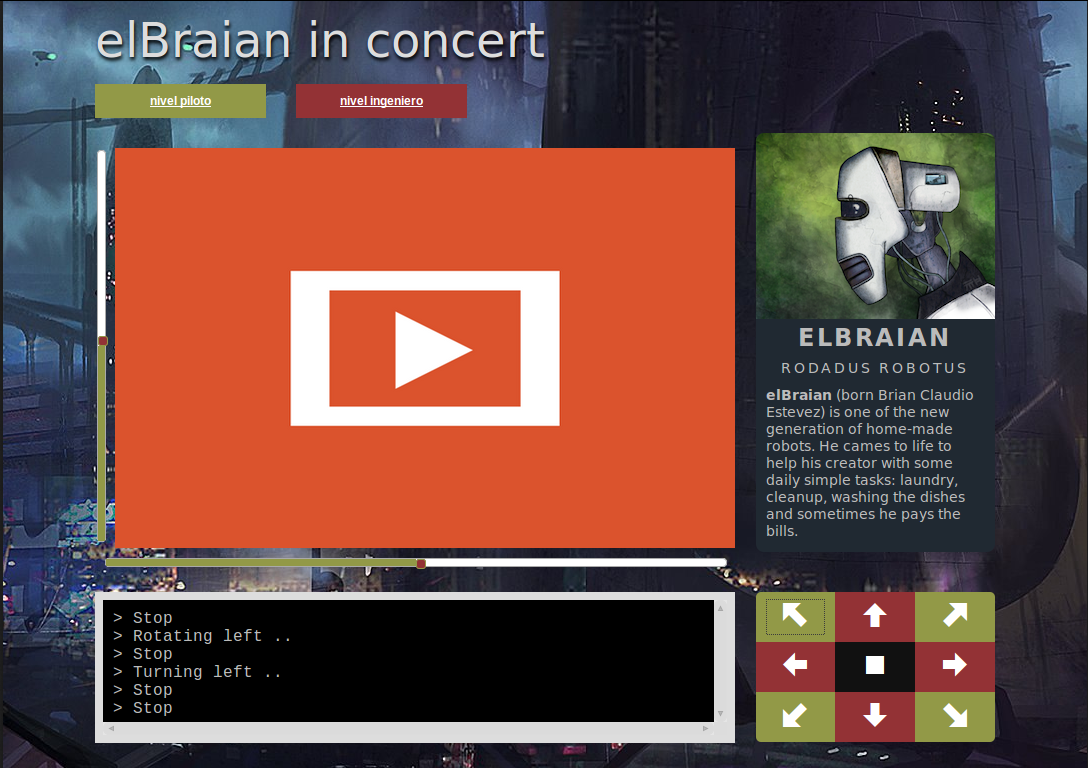
\includegraphics[width=0.5\textwidth]{figures/elbrian-1}
    \caption{Pantalla principal de elBrian (en el recuadro rojo normalmente
        se muestra la cámara de el robot)}
    \label{fig:elbrian}
\end{figure}

Las tecnologías utilizadas en la interfaz web de ``elBrian'' coinciden en gran
parte con las utilizadas en el desarrollo de XRemoteBot, pero el objetivo del
servidor de ``elBrian'' es controlar un único robot en un ambiente local,
además este servidor
se instala en el robot cuestión que sería imposible en los robots basados en
microcontroladores AVR y PIC (``Basic Stamp 2`` de Parallax)
a los que XRemoteBot se encuentra dirigido.


El servidor web de ``elBrian'' está implementado usando el framework Tornado,
WebSockets, mjpg-streamer, opencv y JSON. El mismo está diseñado para ejecutarse
en el robot ya que el mismo está basado en una placa RaspberryPi, la cuál
cuenta con un procesador ARM perfectamente capaz de ejecutar un sistema
operativo completo como GNU/Linux y de soportar el intérprete oficial de Python.

Mientras que este servidor coincide en gran medida en la elección de lenguaje
y bibliotecas utilizadas su implementación es específica para el robot ``elBrian''
y no podría ser portada para robots con menores capacidades de procesamiento
sin una reescritura significativa. Además el protocolo utilizado no contempla
el acceso a valores de sensores, los únicos mensajes que permite enviar
al robot son movimientos.

\begin{itemize}
    \item Educabot \url{http://www.educabot.org/}
    \item Código fuente de ``elBrian'' \url{https://github.com/educabot/elBraian}
\end{itemize}

\section{Gobot con cppp-io}

Gobot~\footnote{\url{http://gobot.io}}
es una biblioteca que permite controlar robots programando en el lenguaje
Go~\footnote{\url{https://golang.org/}}, esta biblioteca soporta el
protocolo Firmata~\footnote{\url{https://github.com/firmata/protocol}}
para controlar robots
conectados directamente a través de una interfaz serial, como es el caso
de los robots Multiplo N6, y soporta la API
cppp-io~\footnote{\url{https://github.com/hybridgroup/cppp-io/}}
que define una API JSON
que permite el acceso a la información y control de robots a través de la Web.

Gobot además tiene compatibilidad con distintos sensores y robots, además de
ser compatible con
placas utilizadas normalmente en la construcción de robots como Arduino,
Raspberry Pi, Intel Edison y Beaglebone Black.

Este proyecto es interesante como base para desarrollar algún proyecto
similar a XRemoteBot en Go, pero requeriría además la reimplementación
del módulo de Python DuinoBot que controla, a través de una versión
modificada del protocolo Firmata, a los robots Multiplo N6 y por otro
lado los robots Scribbler tampoco aparecen en la lista de robots soportados.

\section{Tele Toyland}

Este sitio provee acceso a varios dispositivos a través de una interfaz
Web~\footnote{\url{http://www.teletoyland.com}}
por ejemplo es posible controlar un cabezal con una punta que dibuja sobre
una caja de arena, basta con hacer clic sobre las posiciones sobre las cuales
se quiere que pase la punta y presionar el botón ``go'' para que el cabezal
empiece a moverse dibujando lo pedido, en este y el resto de los experimentos
disponibles en el sitio los resultados se pueden ver a través de un streaming
de video.

Entre los proyectos con los que permite interactuar Tele Toyland
hay 2 areneros como el descripto
anteriormente, una torre de leds, una marioneta y laberintos.

El sitio no provee detalles del software, ni el protocolo utilizado. Desde
lo funcional
provee una especie de control remoto para los distintos dispositivos a los
que permite
manipular, se puede incluso configurar una serie de instrucciones a ejecutar
en secuencia. Sin embargo no provee una biblioteca que permita controlar
los dispositivos desde un lenguaje de programación.


% FIXME
%\section{}
%http://www3.uji.es/~pnebot/Files/Articuls/RemoteProgramming.pdf
%Otro
%http://telerobot.mech.uwa.edu.au/Telerobot/instructions.html
\section{DIY}
% www.linuxuser.co.uk/tutorials/control-your-raspberry-pi-robot-from-a-web-connected-device
Finalmente en la consigna de ``do it yourself'' existen diversas guías para
programar servidores que permitan controlar robots o microcontroladores
en general, se puede encontrar un caso muy bien explicado en el sitio
de Adafruit~\url{https://learn.adafruit.com/wifi-controlled-mobile-robot/building-the-web-interface},
este es un buen ejercicio de programación, sobre todo para aprender a
programar servidores que provean una API web y clientes que la consuman. Sin
embargo estas guías son introductorias y el objetivo es crear un servidor
muy simple, similar a lo que fue el servidor RemoteBot, pensados para ser
usados en un ambiente local ya que no proveen autenticación en general.

